%% \documentclass[9pt,french]{beamer}
%% \usepackage[utf8]{inputenc}
%% \usepackage[T1]{fontenc}

%% \usepackage{amsmath}
%% \usepackage{amsfonts}
%% \usepackage{amssymb}
%% \usepackage{xcolor}
%% \usepackage{alltt}
%% \usepackage{textcomp}
%% \usepackage{mathrsfs}
%% \usepackage{stmaryrd}
%% \usepackage{subfig}
%% \usepackage{listings}
%% \usepackage{pgf}
%% \usepackage{graphicx}
%% \usepackage{enumitem}

%% \usepackage{tikz}
%% \usetikzlibrary{calc,arrows,patterns,plotmarks,shapes,snakes,er,3d,automata,backgrounds,topaths,trees,petri,mindmap}
%% \usepackage{pgfplots}
%% \usepackage{pgfplotstable}

%% %%% For code c++ environment
%% \definecolor{blue_code}{RGB}{106, 90, 205}
%% \definecolor{grey_comment}{RGB}{105, 105, 105}
%% \lstset{
%% language = c++,
%% basicstyle = \footnotesize,
%% numberstyle = \footnotesize,
%% aboveskip=\smallskipamount,
%% showspaces=false,
%% showstringspaces=false,
%% backgroundcolor=\color{blue_code!20},
%% commentstyle=\color{grey_comment},
%% morecomment=[l]{//},
%% frame = single
%% }
%% %%%%
%% \usetheme{CambridgeUS}

%% \title[SEME 2014 - cerema 2]{Utilisation de l'équation de transport pour la prévision du bruit}
%% \subtitle{Vers un nouveau modèle d'acoustique du batiment}

%% \author[shortname]{author1 \inst{1} \and author2 \inst{2}}
%% \institute[shortinst]{\inst{1} affiliation for author1 \and %
%%                       \inst{2} affiliation for author2}

%% %\titlegraphic{
\includegraphics[width=4cm]{Figures/logo-cerema.jpg} }

%% \AtBeginSection[]{
%%    \begin{frame}
%%    \tableofcontents[currentsection,hideothersubsections]
%%    \end{frame} 
%% }

%% \begin{document}

%% \begin{frame}
%% \titlepage
%% \end{frame}

\scriptsize

\begin{frame}
\frametitle{Géometrie du problèmè : notations}
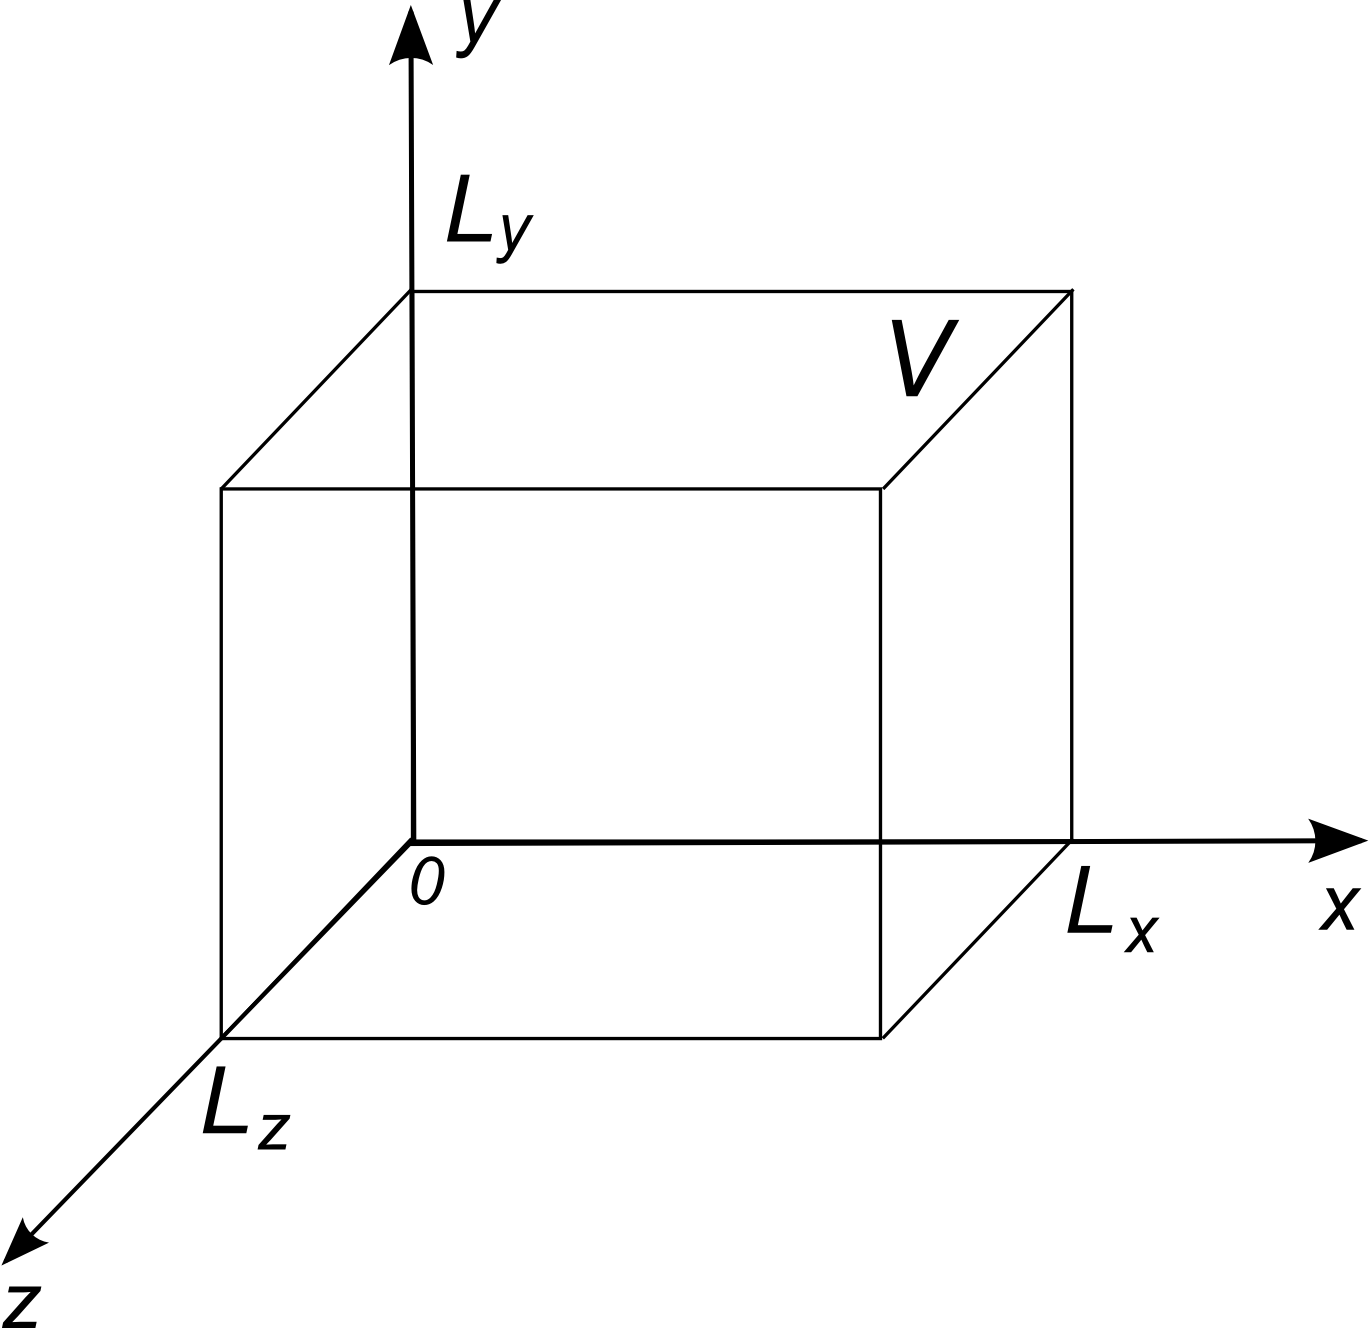
\includegraphics[scale=0.5]{Figures/cube_seme.png}\hspace{1cm}
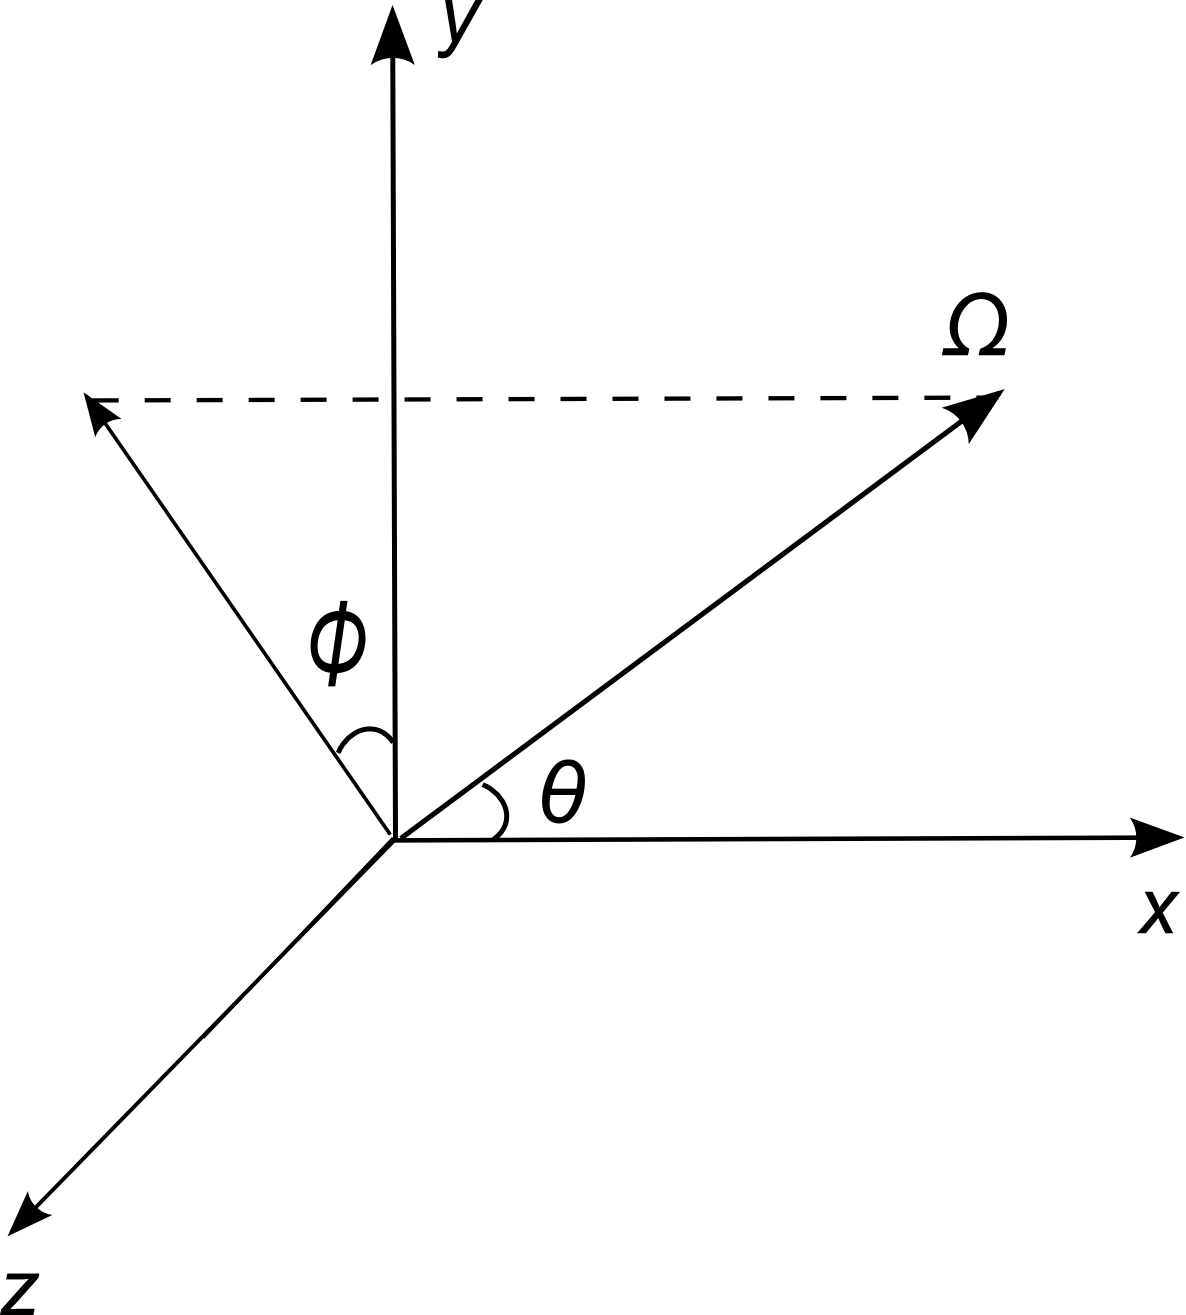
\includegraphics[scale=0.45]{Figures/vitesse_seme.png}
\end{frame}

\begin{frame}
\frametitle{Motivation}
Y. Jing, E. W. Larsen, N. Xiang, 2010 : Cas d'un \textbf{couloir} ($L_y<<L_x$, $L_z<<L_x$)
\begin{itemize}
\item Décomposition $w(\textbf{r}, \theta, \phi, t)=\sum\limits_{j\in\mathbb{N}}\beta_j(y,z,\phi)w_j(x,\theta,t)$ 
\item $\quad\Rightarrow\quad$ réduction du problème : 
\begin{multline*}
\frac{\partial w_{j}(x,\theta,t)}{\partial t}=-\left(\cos{\theta}\frac{\partial w_{j}(x,\theta,t)}{\partial x}+\sin{\theta}\sum\limits_{i\in\mathbb{N}}a_{ij}w_{i}(x,\theta,t)\right.\\
\left.+\sin{\theta}\sum\limits_{i\in\mathbb{N}}b_{ij}\int\limits_{0}^{\pi}\sin^2{\theta'}w_{i}(x,\theta',t)d\theta'\right)
-Mv w_{j}(x,\theta,t)+w^{sce}_{j}(x,\theta,t),\qquad j\in\mathbb{N}
\end{multline*}
\end{itemize}
\begin{minipage}{8cm}
\begin{itemize}
\item Hypothèse : $\beta_j(y,z,\phi)=\beta_j(D(y,z,\phi))$,\quad $j\in\mathbb{N}$
\end{itemize}
\vspace{1.5cm}
\end{minipage}
\hspace{0.5cm}
\begin{minipage}{3cm}
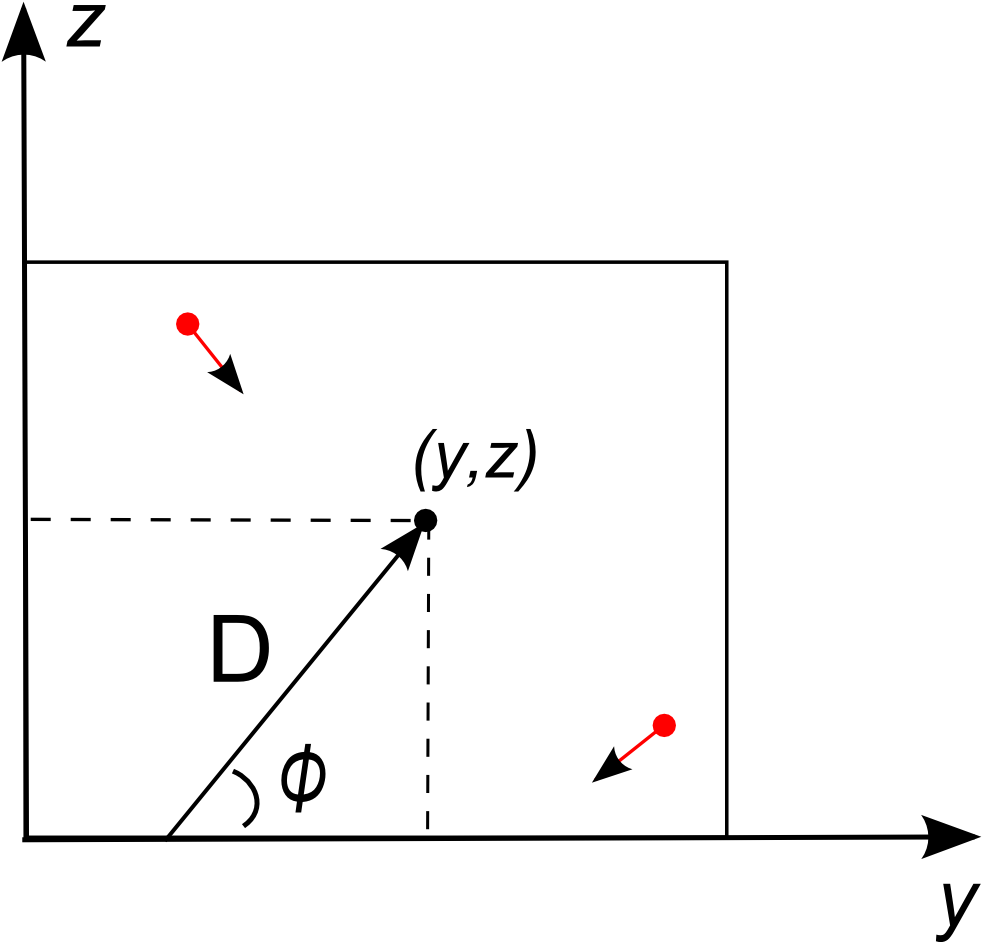
\includegraphics[scale=0.3]{Figures/D_seme.png}
\end{minipage}

Trouver une décomposition pour une \textbf{salle homogène}
\begin{itemize}
\item en espace ? en vitesse ? quelle base ?
\end{itemize}
\end{frame}

\begin{frame}
\frametitle{Décomposition en fonctions sphériques}
On propose de décomposer la fonction $w(\textbf{r},\theta,\phi,t)$ en harmoniques sphériques $Y_{l,m}(\theta,\phi)$.

Harmoniques sphériques :
\begin{equation*}
Y_{l,m}(\theta,\phi)=\sqrt{\frac{2l+1}{2}\frac{(l-m)!}{(l+m)!}}P_{l,m}(cos{\theta})e^{im\phi}
\end{equation*}
Polyn\^omes de Legendre associés :
\begin{equation*}
P_{l,m}(x)=(1-x^2)^{m/2}\frac{d^{m+l}}{dx^{m+l}}(x^2-1)^l, \qquad 0\leqslant m\leqslant l,
\end{equation*}
\begin{equation*}
P_{l,-m}(x)=(-1)^m\frac{(l-m)!}{(l+m)!}P_{l,m}(x)
\end{equation*}
Décomposition de $w(\textbf{r},\theta,\phi,t)$ :
\begin{equation}\label{decomposition}
w(\textbf{r},\theta,\phi,t)=\sum\limits_{l\in\mathbb{N}}\sum\limits_{|m|\leqslant l}w_{l,m}(\textbf{r},t)Y_{l,m}(\theta,\phi)
\end{equation}
\end{frame}

\begin{frame}
\frametitle{Décomposition en harmoniques sphériques}
Après avoir injecté (\ref{decomposition}) dans l'équation (\ref{}), en mulpipliant par $\overline{Y}_{q,p}(\theta,\phi)$ et en intégrant sur la sphère $(\theta,\phi)\in\mathbb{S}^2$ on obtient :

\medskip
\fbox{
\begin{minipage}{0.98\textwidth}
\begin{multline*}
\frac{\partial w_{q,p}(\textbf{r},t)}{\partial t}=-\sum\limits_{l\in\mathbb{N}}\sum\limits_{|m|\leqslant l}\left(B^x_{qplm}\frac{\partial w_{l,m}(\textbf{r},t)}{\partial x}+B^y_{qplm}\frac{\partial w_{l,m}(\textbf{r},t)}{\partial y}+B^z_{qplm}\frac{\partial w_{l,m}(\textbf{r},t)}{\partial z}\right)\\
-Mvw_{q,p}(\textbf{r},t)+w^{sce}_{q,p}(\textbf{r},t),\qquad \textbf{r}\in V,\quad q\in\mathbb{N},\quad |p|\leqslant q
\end{multline*}
\end{minipage}}
\medskip

Condition au bord multipliée par $\overline{Y}_{q,p}(\theta,\phi)$ et integrée sur la demi-sphère ${\Omega}\cdot\mathbf{n}<0$ donne :

\medskip
\fbox{
\begin{minipage}{0.8\textwidth}
\begin{equation*}
\sum\limits_{l\in\mathbb{N}}\sum\limits_{|m|\leqslant l}\Gamma_{qplm}(\mathbf{r})w_{l,m}(\mathbf{r},t)=0,\qquad \mathbf{r}\in\partial V,\quad q\in\mathbb{N},\quad |p|\leqslant q
\end{equation*}
\end{minipage}}

\medskip
Les matrices $B^x$, $B^y$ et $B^z$ sont hermitiennes : $B^x=(B^x)^*$, $B^y=(B^y)^*$, $B^z=(B^z)^*$.
\smallskip
\begin{equation*}
B^x_{qplm}=\sqrt{\frac{q^2-p^2}{4q^2-1}}\delta_{q-1,l}\delta_{p,m}+\sqrt{\frac{(q+1)^2-p^2}{4(q+1)^2-1}}\delta_{q+1,l}\delta_{p,m},
\end{equation*}
\end{frame}

\begin{frame}
\frametitle{Décomposition en harmoniques sphériques}
\begin{multline*}
B^y_{qplm}=\left(\frac{1}{\sqrt{2q-1}}\sqrt{(q+p)(q+p-1)}\delta_{q-1,l}\delta_{p-1,m}\right.\\
-\frac{1}{\sqrt{2q-1}}\sqrt{(q-p)(q-p-1)}\delta_{q-1,l}\delta_{p+1,m}\\
-\frac{1}{\sqrt{2q+3}}\sqrt{(q-p+2)(q-p+1)}\delta_{q+1,l}\delta_{p-1,m}\\
\left.+\frac{1}{\sqrt{2q+3}}\sqrt{(q+p+2)(q+p+1)}\delta_{q+1,l}\delta_{p+1,m}\right)\frac{1}{2\sqrt{2q+1}},
\end{multline*}
\begin{multline*}
B^z_{qplm}=\frac{1}{2i\sqrt{2q+1}}\left(\frac{1}{\sqrt{2q-1}}\sqrt{(q+p)(q+p-1)}\delta_{q-1,l}\delta_{p-1,m}\right.\\
+\frac{1}{\sqrt{2q-1}}\sqrt{(q-p)(q-p-1)}\delta_{q-1,l}\delta_{p+1,m}\\
-\frac{1}{\sqrt{2q+3}}\sqrt{(q-p+2)(q-p+1)}\delta_{q+1,l}\delta_{p-1,m}\\
\left.-\frac{1}{\sqrt{2q+3}}\sqrt{(q+p+2)(q+p+1)}\delta_{q+1,l}\delta_{p+1,m}\right).
\end{multline*}
\end{frame}
\begin{frame}
\frametitle{Décomposition en harmoniques sphériques}
Sur la frontière $y=0$ :
\begin{multline*}
\Gamma^{y=0}_{qplm}=\frac{\sin{\left((m-p)\pi/2\right)}}{m-p}T_{qplm}-R(1-s)(-1)^m\frac{\sin{((m+p)\pi/2)}}{m+p}T_{qplm}+\\
(-1)^m\frac{2s}{\pi}\frac{\sin{(p\pi/2)}}{p}\frac{\cos{(m\pi/2)}}{m^2-1}Q_{qp}\\
\times\left(Q_{l+1,m+1}\sqrt{\frac{(l+m+2)(l+m+1)}{(2l+3)(2l+1)}}-Q_{l-1,m+1}\sqrt{\frac{(l-m-1)(l-m)}{(2l-1)(2l+1)}}\right).
\end{multline*}

où

\begin{equation*}
T_{qplm}=\frac{1}{4\pi}\sqrt{(2q+1)(2l+1)}\sqrt{\frac{(q-p)!}{(q+p)!}\frac{(l-m)!}{(l+m)!}}\int\limits_{-1}^1P^p_q(x)P^m_l(x)dx,
\end{equation*}
\begin{equation*}
Q_{qp}=\frac{1}{\sqrt{4\pi}}\sqrt{2q+1}\sqrt{\frac{(q-p)!}{(q+p)!}}\int\limits_{-1}^1P^p_q(x)dx.
\end{equation*}
\end{frame}
%%\section{Approche numérique}

\subsection{Transport avec une direction fixée pour $\vec{v}$}
\begin{frame}{Equation de transport - Discrétisation}

  \begin{block}{Equation de transport}
    \begin{equation*}
      \frac{\partial w(\vec{r}, \theta, \phi, t)}{\partial t} = -\vec{v} \cdot \nabla w(\vec{r}, \theta, \phi, t) - M v w(\vec{r}, \theta, \phi, t) + 
      w_{sce}(\vec{r}, \theta, \phi, t)
    \end{equation*}
    
    \begin{columns}[c]
      \begin{column}{5cm}
        \begin{itemize}
        \item $\vec{r} : (x_1,...,x_{dim})$ \\
          1D,2D, ou 3D en espace
        \end{itemize}
      \end{column}
      \begin{column}{5cm}
        \begin{itemize}
        \item $\vec{v} : (\theta, \phi)$ \\
          2D pour les directions
        \end{itemize}
      \end{column}
    \end{columns}

    \begin{center}
      \textcolor{red}{Modèle 5D instationnaire}
    \end{center}
  \end{block}

  \begin{alertblock}{Discrétisation : Schéma différence finies implicite centré}
    \begin{columns}[c]
      \begin{column}{6cm}
        \begin{equation*}
          \frac{\partial w}{\partial t} = \frac{w^{t+1}_{\vec{r}} - w^t_{\vec{r}}}{\Delta t}
        \end{equation*}
      \end{column}
      \begin{column}{6cm}
        \begin{equation*}
          \frac{\partial w}{\partial x_i} = \frac{w^{t+1}_{r_i + 1} - w^{t+1}_{r_i - 1}}{2\Delta x_i}
        \end{equation*}
      \end{column}
    \end{columns} 

  \end{alertblock}

\end{frame}

\begin{frame}{Schéma aux différences finies}
  \begin{equation*}
    \frac{w_{\vec{r}}^{t+1} - w_{\vec{r}}^{t}}{\Delta t} + 
    \sum \limits_{i=1}^{Dim} v_i \left( \frac{w_{r_i+1}^{t+1} - w_{r_i-1}^{t+1}}{2 \Delta x_i} \right)
    + Mvw_{\vec{r}}^{t+1} = w_{sce}
  \end{equation*}

  %forme matricielle
  \begin{columns}[c]
    \begin{column}{5cm}
      \centering
      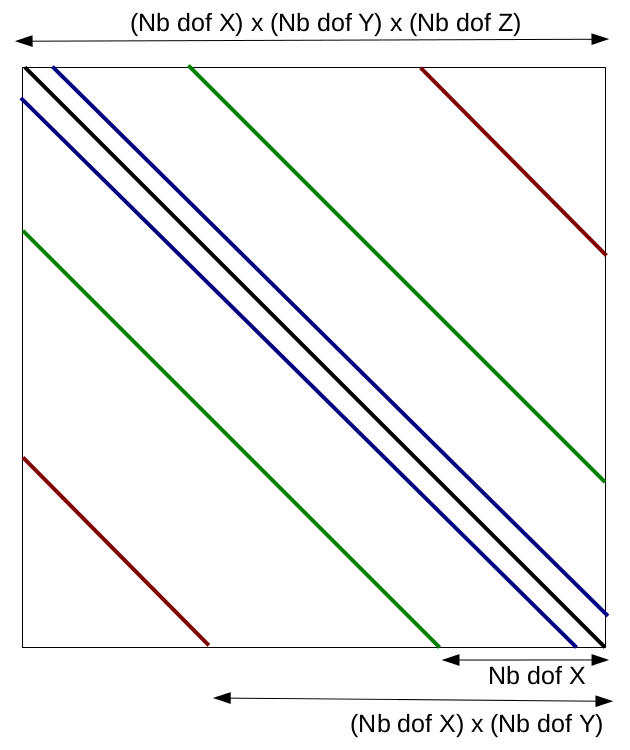
\includegraphics[scale=0.3]{Figures/FD_matrix.png}
    \end{column}
    \begin{column}{6.5cm}
      \begin{itemize}[label=$\rightarrow$]
      \item \textcolor{black}{$\bullet$} terme diagonal : $\frac{1}{\Delta t} + Mv$
      \item \textcolor{blue}{$\bullet$} schéma centré en $x$ : $\pm \frac{v_x}{2\Delta x}$
      \item \textcolor{green}{$\bullet$} schéma centré en $y$ : $\pm \frac{v_y}{2\Delta y}$
      \item \textcolor{red}{$\bullet$} schéma centré en $z$ : $\pm \frac{v_z}{2\Delta z}$
      \end{itemize}
    \end{column}
  \end{columns} 

\end{frame}

\begin{frame}
  Video 1D Dirichlet homogene sans stabilisation
\end{frame}

\begin{frame}{Stabilisation : ajout d'un terme de diffusion artificiel}
  %Stabilisation : ajout d'un terme de diffusion artificiel
  \vspace*{-0.6cm}
  \begin{eqnarray*}
    \frac{\partial w(\vec{r}, \theta, \phi, t)}{\partial t} &=& -\vec{v} \cdot \nabla w(\vec{r}, \theta, \phi, t) - M v w(\vec{r}, \theta, \phi, t) + 
    w_{sce}(\vec{r}, \theta, \phi, t) \\
    &+& \text{ \textcolor{red}{$\nabla (\tau_{art} \nabla w(\vec{r}, \theta, \phi, t))$} } 
    \qquad \tau_{art} = \frac{\rho h \prod \limits_{i=1}^{Dim} v_i }{\parallel \vec{v} \parallel}
  \end{eqnarray*}

  %avec $\tau_{art} = \frac{\rho h \prod \limits_{i=1}^{Dim} v_i }{\parallel \vec{v} \parallel}$

  \vspace*{-0.3cm}
  %forme matricielle
  \begin{columns}[c]
    \begin{column}{4.5cm}
      \centering
      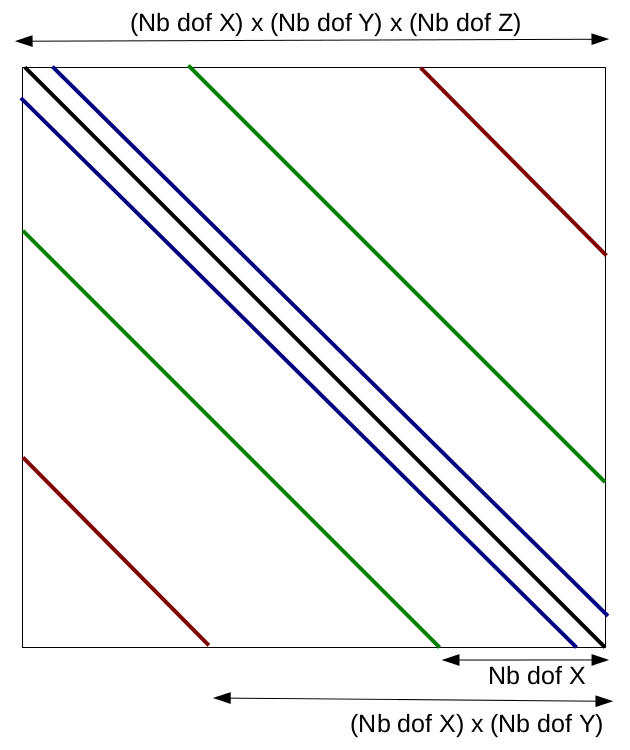
\includegraphics[scale=0.26]{Figures/FD_matrix.png}
    \end{column}
    \begin{column}{7.5cm}
      \begin{itemize}[label=$\rightarrow$]
      \item \textcolor{black}{$\bullet$} terme diagonal : $\frac{1}{\Delta t} + Mv$ 
        + \textcolor{red}{$\frac{2\tau_{art}}{\Delta x^2} + \frac{2\tau_{art}}{\Delta y^2} + \frac{2\tau_{art}}{\Delta z^2}$}
      \item \textcolor{blue}{$\bullet$} schéma centré en $x$ : $\pm \frac{v_x}{2\Delta x}$
        - \textcolor{red}{$\frac{\tau_{art}}{\Delta x^2}$}
      \item \textcolor{green}{$\bullet$} schéma centré en $y$ : $\pm \frac{v_y}{2\Delta y}$
        - \textcolor{red}{$\frac{\tau_{art}}{\Delta y^2}$}
      \item \textcolor{red}{$\bullet$} schéma centré en $z$ : $\pm \frac{v_z}{2\Delta z}$
        - \textcolor{red}{$\frac{\tau_{art}}{\Delta y^2}$}
      \end{itemize}
    \end{column}
  \end{columns} 

\end{frame}

\begin{frame}
  Video 1D Dirichlet homogene avec stabilisation
\end{frame}

\subsection{Prise en compte de la condition limite}
\begin{frame}{Condition aux limites}

  Sur les bords du domaine (= murs de la salle) :
  \begin{itemize}[label=$\bullet$]
  \item une partie de l'énergie est réfléchie de façon spéculaire %(probabilité $1-d$)
  \item l'autre partie est réfléchie de façon diffuse %(probabilité $d$) \\
    \vspace*{0.2cm}
  \item $R$ (coefficient de réflexion) et $d$ (coefficient de diffusivité) dépendent de la paroi considérée
  \end{itemize}

  \vspace*{-0.4cm}
  \begin{small}
    \begin{equation*}
      w(\vec{r},\theta,\phi,t) = \underbrace{R(1-d)w(\vec{r},\hat{\theta},\hat{\phi},t)}_{\text{reflexion spéculaire}}
      + \underbrace{ \int_{0}^{2\pi} \int_{0}^{\frac{\pi}{2}} Rd\frac{1}{\pi v} \vec{v}'w(\vec{r},\theta',\phi',t) sin \theta' d\theta' d\phi'}_{\text{reflexion diffuse}}
    \end{equation*}
    si $\vec{v} \cdot \vec{n} < 0$ ( $w(\vec{r},\theta,\phi,t)$ = 0 sinon) \\
  \end{small}

  où $\vec{v} \cdot \vec{n} = -\hat{\vec{v}} \cdot \vec{n}$, avec
  \begin{equation*}
    v=
    \left(
    \begin{array}{lll}
      cos(\theta)\\
      sin(\theta)cos(\phi)\\
      sin(\theta)sin(\phi)
    \end{array}
    \right)
    \Rightarrow
    \left \{
    \begin{array}{ll}
      \hat{\theta} = \pi - \theta \\
      \hat{\phi} = \pi - \phi \\
    \end{array}
    \right.
  \end{equation*}
  et $\vec{v} \cdot \vec{n} \neq -\vec{v}' \cdot \vec{n}$
\end{frame}

\subsection{Transport prenant en compte plusieurs directions pour $\vec{v}$}
\begin{frame}{Stratégie}

  \begin{columns}[c]
    \begin{column}{6cm}
      \begin{itemize}[label=$\bullet$]
      \item Directions $(\theta,\phi)$ organisées selon une grille 2D
      \item Resolution 3D pour chaque direction $(\theta,\phi)$
      \item \textbf{Résultat} : somme des densités dans toutes les directions :\\
        $w(\vec{r},t) = \sum \limits_{(\theta,\phi)} w(\vec{r},\theta,\phi,t)$
      \end{itemize}

      \begin{alltt}
        for[ pas de temps $t$ ] \\        
        \hspace*{0.2cm} for[ direction $(\theta,\phi)$ ] \\
        \hspace*{0.4cm} assemblage matrice
        \hspace*{0.4cm} assemblage second membre
        \hspace*{0.4cm} Resolution $\Rightarrow w(\vec{r},\theta,\phi,t)$
        \hspace*{0.4cm} $w(\vec{r},t)$ += $w(\vec{r},\theta,\phi,t)$
      \end{alltt}
    \end{column}
    \begin{column}{6.5cm}
      \begin{figure}[H]
        \centering
        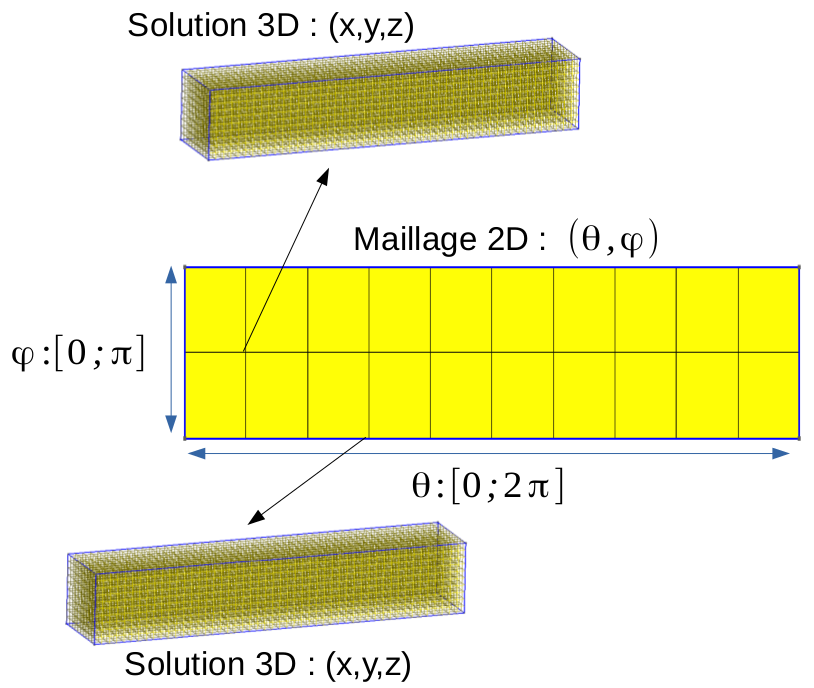
\includegraphics[scale=0.32]{Figures/Schema_mesh.png}
      \end{figure}
    \end{column}
  \end{columns}
\end{frame}



%%\end{document}
